% !Mode:: "TeX:UTF-8"
\documentclass{article}
\usepackage[hyperref, UTF8]{ctex}
\usepackage[dvipsnames]{xcolor}
\usepackage{geometry}
\usepackage{amsmath}
\usepackage{amsfonts}
\usepackage[section]{placeins}
\usepackage{listings}
\usepackage{pgfplotstable}
\usepackage{pgfplots}
\usepackage{fontspec}
\usepackage{comment}
\usepackage{booktabs} % 表格上的不同横线
\setmonofont[Mapping={}]{Consolas}	%英文引号之类的正常显示,相当于设置英文字体
\setsansfont{Consolas} %设置英文字体 Monaco, Consolas,  Fantasque Sans Mono
\setmainfont{Consolas} %设置英文字体

\definecolor{mygreen}{rgb}{0,0.6,0}
\definecolor{mygray}{rgb}{0.5,0.5,0.5}
\definecolor{mymauve}{rgb}{0.58,0,0.82}
\lstset{ %
    backgroundcolor=\color{white},   % choose the background color
    basicstyle=\footnotesize\ttfamily,        % size of fonts used for the code
    columns=fullflexible,
    breaklines=true,                 % automatic line breaking only at whitespace
    captionpos=b,                    % sets the caption-position to bottom
    tabsize=4,
    backgroundcolor=\color[RGB]{245,245,244},            % 设定背景颜色
    commentstyle=\color{mygreen},    % comment style
    escapeinside={\%*}{*)},          % if you want to add LaTeX within your code
    keywordstyle=\color{blue},       % keyword style
    stringstyle=\color{mymauve}\ttfamily,     % string literal style
    showstringspaces=false,                % 不显示字符串中的空格
    frame=none,
    rulesepcolor=\color{red!20!green!20!blue!20},
    % identifierstyle=\color{red},
    language=sql,
}

% 设置hyperlink的颜色
\newcommand\myshade{85}
\colorlet{mylinkcolor}{violet}
\colorlet{mycitecolor}{YellowOrange}
\colorlet{myurlcolor}{Aquamarine}

\hypersetup{
  linkcolor  = mylinkcolor!\myshade!black,
  citecolor  = mycitecolor!\myshade!black,
  urlcolor   = myurlcolor!\myshade!black,
  colorlinks = true,
}

\renewcommand\figurename{图}

\setcounter{secnumdepth}{5}

\title{软件工程大作业文档}
\author{Tomato}
\date{2018年1月}

\begin{document}

\maketitle
\section{系统/子系统设计(结构设计)说明(后台部分)}
\subsection{引言}
\subsubsection{系统概述}
后台分为两个部分,上层是Controller,是用来处理业务逻辑的,下层是数据库,给上层的Controller提供相应的服务。下面会分两块来具体介绍这两部分。详见\ref{接口设计说明}和\ref{数据库(顶层)设计说明}。

\subsubsection{文档概述}
本文档将围绕Spring Boot架构来介绍后台部分。
\subsection{系统级设计决策}
本系统后台主要使用Spring Boot架构,它支持在开启服务的时候,接受HttpRequest或websocket并进行后台处理,然后返回相应的结果。系统接受的输入是HttpRequest或websocket,详见\ref{接口设计说明},对于每一个输入的响应,被Controller定义,不同的request会有不同的Controller 对其进行处理并返回相应的结果。系统处理的过程中,依赖于两部分的内容:用户的request中的具体内容和底层数据库已有的信息。详见\ref{数据库(顶层{设计说明}}。该系统的数据库存在服务器上,服务器的管理人员可以通过database asdan来访问数据库并查看当前数据库中的所有信息。该系统对服务器的要求是要求服务器能通过maven运行项目,并配有mysql数据库。
\subsection{系统体系结构设计}
\subsubsection{系统总体设计}
\paragraph{概述}
	%unfinished
	本系统要实现的功能详见《prj9ASDAN模拟商业竞拍交易大赛系统》。本系统要实现的性能:响应较快、支持并发、有一定的安全性、可在各个平台上运行、可移植等。本系统支持在Windows、Unix、Linux环境下运行。
\paragraph{设计思想}
	本系统顶层核心要处理的两个问题是对于HttpRequest的处理和对于websocket的处理,而底层核心要处理的问题是数据库的维护等问题。如果直接从头开始开发一套框架,则要实现的内容可能比我们当前写的多得多。所以我们后台根据这个需求找到了Spring Boot框架。Spring Boot 很好地通过了Annotations来实现我们需要的对于前端web端的响应,也实现了我们需要的和数据库的连接、并发的响应等等。本系统并不需要很高深的算法,但是对逻辑上的要求十分的多和细致。
\paragraph{基本处理流程}
	%unfinished 需要画图
\paragraph{系统体系结构}
	%unfinished 需要画图
\paragraph{功能需求与系统配置项的关系}
	%unfinished 需要画图
\subsubsection{执行概念}
%unfinished 需要画图
\subsubsection{接口设计}
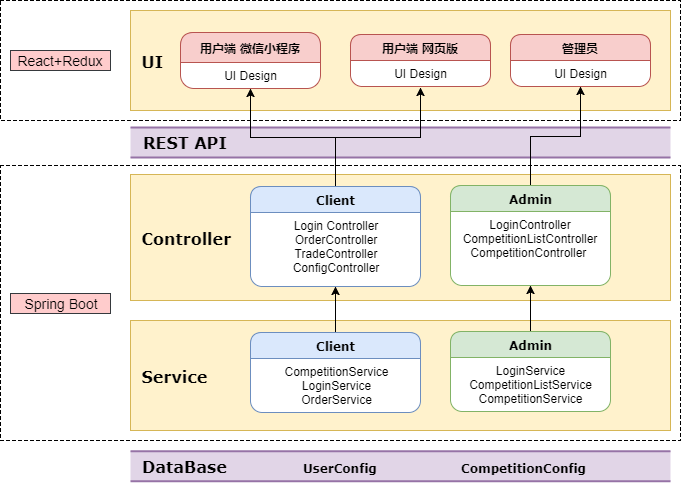
\includegraphics[scale = .3]{架构图.png}
\subsection{系统出错处理设计}
系统出错后,后台数据库的内容不会被清空,并且我们是在处理request流程中对数据库是实时更新的,宕机之后数据库的内容还是会保留,当下次启动服务器的时候它还能从原数据库中获得原来的数据,并根据这些数据进行处理。

当系统出错后,建议重启服务器。
\subsection{尚待解决的问题}
微信后端的websocket的测试问题。
\subsection{需求的可追踪性}
\subsection{注解}

\section{接口设计说明}
\label{接口设计说明}
\subsection{引言}
\subsubsection{系统概述}
接口主要分为两大类的接口,一类是Admin的接口,另一类是Client的接口。Client有两种接口,一种是web端的接口,另一类是微信端的接口。Admin本身是一个package,两种Client公用一个package,名为client。Web端的接口包括了正常HttpRequest和Web端的Websocket。Web端的Websocket使用StompClient协议,在后端使用Spring Boot自带的Controller,即@MessageMapping和@SendTo来完成对socket内容的转发。而微信端在HttpRequest上和Web端共用一个API,并使用裸的socket来回复websocket。
\subsubsection{文档概述}
文档首先介绍了使用的文献,然后对于每个特定的接口进行了具体的说明。
\subsection{引用文件}
本文档引用了我们在开发过程中撰写的《RestAPI》文档,详情可查看\href{https://github.com/wenj/tomatodesign/blob/master/REST%20API.tex}{RestAPI.tex}。

\subsection{Admin接口}

\subsubsection{Login Admin}
管理员登录。

\paragraph*{Request}
\begin{lstlisting}
POST /api/admin/login

Host: localhost:8080
Auth:
Content-type: application/json
Accept: application/json

{
    "username": "admin",
    "password": "admin",
}
\end{lstlisting}

\paragraph*{Returns}
\begin{lstlisting}
HTTP 200 OK
{
    "username": "admin",
    "token": "1283091828021803120",
}

\end{lstlisting}

\paragraph*{Error}
\begin{lstlisting}
HTTP 401 NOTAUTHORIZED
{
    "error": "Admin with username admin doesn\'t exist or password is wrong."
}
\end{lstlisting}

\subsubsection{Change Admin Password}
更改管理员密码。

\paragraph*{Request}
\begin{lstlisting}
POST /api/admin/update

Host: localhost:8080
Auth:
Content-type: application/json
Accept: application/json

{
    "username": "admin",
    "prePassword": "admin",
    "newPassword": "newpwd",
}
\end{lstlisting}

\paragraph*{Returns}
\begin{lstlisting}
HTTP 200 OK

\end{lstlisting}

\paragraph*{Error}
\begin{lstlisting}
HTTP 401 NOTAUTHORIZED
{
    "error": "Wrong password of admin."
}
\end{lstlisting}


\subsubsection{Get All Competitions}

列出全部比赛。

Status是"not\_start", "auction\_not\_record", "auction\_recorded", "trade", "rest", "end"之一。

\paragraph*{Request}
\begin{lstlisting}
GET /api/admin/competition/getall

Host: localhost:8080
Auth:
Content-type: application/json
Accept: application/json
\end{lstlisting}

\paragraph*{Returns}
\begin{lstlisting}
HTTP 200 OK

[
    {
        "id": "competiton1_id",
        "username": "competition1",
        "status": "auction"
    },
    {
        "id": "competiton2_id",
        "username": "competition2",
        "status": "end"
    }
]
\end{lstlisting}

\paragraph*{Error}
\begin{lstlisting}
HTTP 204 NO CONTENT
\end{lstlisting}

\subsubsection{Create Competition}
新建一场比赛。注意,底层也要生成机器的id。注意每场比赛的基本配置(比赛名称,参赛人数)只能创建一次,不能修改。

\paragraph*{Request}
\begin{lstlisting}
POST /api/admin/competition/new

Host: localhost:8080
Auth:
Content-type: application/json
Accept: application/json

{
    "username": "competition_username",
    "round": 2,
    "startWealth": 1000,

    "teamNum": 2,
    "participantNum": 3,
    "team":
    [
        {
            "username": "team1",
            "participant": ["mem11", "mem12", "mem13"],
            "password": "111111",
        },
        {
            "username": "team2",
            "participant": ["mem21", "mem22", "mem23"],
            "password": "222222",
        }
    ]

    "roundParameter":
    [
        {
            "machineStartPrice": [300, 350, 400],
            "machineNum": [1, 1, 1],
            "materialProduceCost": [10, 20, 30],
            "time": 900,
        },
        {
            "machineStartPrice": [300, 350, 400],
            "machineNum": [1, 1, 1],
            "materialProduceCost": [10, 20, 30],
            "time": 900,
        }
    ]
}
\end{lstlisting}

\paragraph*{Returns}
\begin{lstlisting}
HTTP 201 CREATED

\end{lstlisting}

\paragraph*{Error}
\begin{lstlisting}
HTTP 404 NOT FOUND
{
    "error":"Unable to delete. Competition with id xxx not found."
}
\end{lstlisting}


\subsubsection{Delete Competition By ID}

通过ID删除比赛。

\paragraph*{Request}
\begin{lstlisting}
DELETE /api/admin/competiton/id={competition_id}

Host: localhost:8080
Auth:
Content-type: application/json
Accept: application/json
\end{lstlisting}

\paragraph*{Returns}
\begin{lstlisting}
HTTP 200 OK
[
    {
        "id": "competiton2_id",
        "username": "competition2",
        "status": "end"
    }
]
\end{lstlisting}

\paragraph*{Error}
\begin{lstlisting}
{
    "error":"Unable to delete. Competition with id xxx not found."
}
\end{lstlisting}

\subsubsection{Update Competition Status}

需要进入下一环节时,管理员端会向服务器发送更新比赛状态的请求,服务器返回当前比赛信息以便管理员端更新到最新的比赛状态。

\paragraph*{Web Socket}
\begin{lstlisting}
MessageMapping: /api/admin/status/update/id=3

SendTo: /api/admin/status/id=3

EndPoint:  http://127.0.0.1:8090/competitionStatus

Send JSON Pattern:
{
    "status": "auction"("not_start", "auction_not_record", "auction_recorded", "trade", "rest", "end")
    "round": 0/1/2/3
    "timeLeft":227(s)
 }

Get JSON Pattern:
{
    "status": "auction"("not_start", "auction_not_record", "auction_recorded", "trade", "rest", "end")
    "round": 0/1/2/3
}
\end{lstlisting}

\paragraph*{Error}
\begin{lstlisting}
HTTP 404 NOT FOUND
{
    "error":"Unable to update. Competition with id xxx not found"
}
\end{lstlisting}

\subsubsection{Get Auction Machine}

获得某场比赛某一轮拍卖机器的初始信息。

\paragraph*{Request}
\begin{lstlisting}
GET /api/admin/competition/auction/id={id}/round={round}

Host: localhost:8080
Auth:
Content-type: application/json
Accept: application/json
\end{lstlisting}

\paragraph*{Returns}
\begin{lstlisting}
HTTP 200 OK
[
    {
        "machineId": "machine1",
        "type": "Wood",
        "startPrice": 200,
    },
    {
        "machineId": "machine2",
        "type": "Brick",
        "startPrice": 300,
    },
    {
        "machineId": "machine3",
        "type": "Cement",
        "startPrice": 400,
    }
]
\end{lstlisting}

\paragraph*{Error}
\begin{lstlisting}
HTTP 404 NOT FOUND
{
    "error": "Competition with id xxx not found." (or Competition with id xxx does not have round xxx)
}
\end{lstlisting}

\subsubsection{Record Auction Result}

登记某场比赛某一轮的拍卖结果。

\paragraph*{Request}
\begin{lstlisting}
POST /api/admin/competition/record/id={id}/round={round}

Host: localhost:8080
Auth:
Content-type: application/json
Accept: application/json
\end{lstlisting}

\paragraph*{Returns}
\begin{lstlisting}
HTTP 200 OK
[
    {
        "machineId": "machine1",
        "teamId": "team1",
        "price": 2000,
    },
    {
        "machineId": "machine2",
        "teamId": "brick",
        "price": 3000,
    },
    {
        "machineId": "machine3",
        "teamId": "cement",
        "price": 4000,
    }
]
\end{lstlisting}

\paragraph*{Error}
\begin{lstlisting}
HTTP 404 NOT FOUND
{
    "error": "Competition with id xxx not found." (or Competition with id xxx does not have round xxx)
}
\end{lstlisting}


\subsubsection{Get Competition Property}

从服务器按id获取某一比赛的各种属性。如果该比赛的属性尚未被设置,则该项为空。属性包括名称、比赛轮数(如果比赛已开始,则不能删除已开始或结束的轮)、比赛各项参数(不能修改已开始或结束的轮的参数)、机器的id等等。

\paragraph*{Request}
\begin{lstlisting}
GET /api/admin/competition/property/id={id}

Host: localhost:8080
Auth:
Content-type: application/json
Accept: application/json
\end{lstlisting}

\paragraph*{Returns}
\begin{lstlisting}
HTTP 200 OK
{
    "id": "competition_id",
    "username": "competition_username",
    "status": "not started",
    "teamNum": 1,
    "participantNum": 2,
    "team":
    [
        {
            "username": "team1",
            "participant": ["member1", "member2", "member2"],
            "password": "password",
        }
    ]
    "round": 1,
    "startWealth": 1000,
    "roundParameter":
    [
        {
            "machineStartPrice": [300, 350, 400],
            "machineNum": [1, 1, 1],
            "materialProduceCost": [10, 20, 30],
            "time": 900,
        }
    ]
}

\end{lstlisting}

\paragraph*{Error}
\begin{lstlisting}
HTTP 404 NOT FOUND
{
    "error": "Competition with id xxx not found."
}
\end{lstlisting}

\subsubsection{Update Competition Property}

更新比赛的各种属性。属性包括名称、比赛轮数(如果比赛已开始,则不能更改)、比赛各项参数(不能修改已开始或结束的轮的参数)。

\paragraph*{Request}
\begin{lstlisting}
PUT /api/admin/competition/property/id={id}

Host: localhost:8080
Auth:
Content-type: application/json
Accept: application/json

{
    "round": 2,
    "startWealth": 1000,
    "round_parameter":
    [
        {
            "machineStartPrice": [300, 350, 400],
            "machineNum": [1, 1, 1],
            "materialProduceCost": [10, 20, 30],
            "time": 900,
        },
        {
            "machineStartPrice": [300, 350, 400],
            "machineNum": [1, 1, 1],
            "materialProduceCost": [10, 20, 30],
            "time": 900,
        }
    ]
}
\end{lstlisting}

\paragraph*{Returns}
\begin{lstlisting}
HTTP 201 CREATED
\end{lstlisting}

\paragraph*{Error}
\begin{lstlisting}
HTTP 404 NOT FOUND
{
    "error": "Competition with id xxx not found."
}
\end{lstlisting}

\begin{lstlisting}
HTTP 400 INVALID REQUEST
{
    "error": "Cannot update competition id xxx with given changes."
}
\end{lstlisting}

\subsubsection{Get Competition Information}
获取当前比赛信息,包括队伍的数量、资产、交易记录、机器的使用情况等。

\paragraph*{Request}
\begin{lstlisting}
GET /api/admin/competition/info/id={id}

Host: localhost:8080
Auth:
Content-type: application/json
Accept: application/json
\end{lstlisting}

\paragraph*{Returns}
\begin{lstlisting}
HTTP 200 OK
{
    "id": "competition_id",
    "username": "competition_username",
    "status": "not_start",
    "round": 2,
    "presentRound": 0,
    "teamInfo":
    [
        {
            "id": "id1",
            "wealth": 100,
            "material": [30, 40, 50],
            "machine":
            [
                 {
                    "id": "machine1_id",
                    "type": "type1",
                    "left": 3
                 },
                 {
                    "id": "machine2_id",
                    "type": "type2",
                    "left": 2
                 }
            ]
        },
        {
            "id": "id2",
            "wealth": 100,
            "material": [30, 40, 50],
            "machine":
            [
                 {
                    "id": "machine1_id",
                    "type": "type1",
                    "left": 3
                 },
                 {
                    "id": "machine2_id",
                    "type": "type2",
                    "left": 2
                 }
            ]
        }
    ],
    "trade_history":
    [
        {
            "time": "yyyy-MM-dd'T'HH:mm:ss.SSS'Z'",
            "sell": "team_id1",
            "buy": "team_id2",
            "content": {"wood": 1},
            "price": 10
        },
         {
            "time": "yyyy-MM-dd'T'HH:mm:ss.SSS'Z'",
            "sell": "team_id1",
            "buy": "team_id2",
            "content": {"machine_wood": 1},
            "price": 20
        }
    ]
}

\end{lstlisting}
content中是wood,brick,cement,machine\_wood,machine\_brick,machine\_cement中的一个。

\paragraph*{Error}
\begin{lstlisting}
HTTP 404 NOT FOUND
{
    "error": "Competition with id 1 not found."
}
\end{lstlisting}

\subsubsection{Record machine owner}
向服务器发送对比赛的更新信息。增加机器、分配财产之类的。

\paragraph*{Request}
\begin{lstlisting}
PUT /api/admin/competition/info/id={id}

Host: localhost:8080
Auth:
Content-type: application/json
Accept: application/json

{
    "round": 2,
    "present_round": 0,
    "team_info":
    [
        {
            "id": "id1",
            "wealth": "100",
            "machine":
            [
                 {
                    "id": "machine1_id",
                    "left": 3
                 },
                 {
                    "id": "machine2_id",
                    "left": 2
                 }
            ]
        },
        {
            "id": "id2",
            "wealth": "100",
            "machine":
            [
                 {
                    "id": "machine1_id",
                    "left": 3
                 },
                 {
                    "id": "machine2_id",
                    "left": 2
                 }
            ]
        }
    ]
}
\end{lstlisting}

\paragraph*{Returns}
\begin{lstlisting}
HTTP 200 OK
{
    "id": "competition_id",
    "username": "competition_username",
    "status": "not started",
    "round": "2",
    "present_round": "0",
    "team_info":
    [
        {
            "id": "id1",
            "wealth": 100,
            "material": [30, 40, 50],
            "machine":
            [
                 {
                    "id": "machine1_id",
                    "type": "type1",
                    "left": 3
                 },
                 {
                    "id": "machine2_id",
                    "type": "type2",
                    "left": 2
                 }
            ]
        },
        {
            "id": "id2",
            "wealth": 100,
            "material": [30, 40, 50],
            "machine":
            [
                 {
                    "id": "machine1_id",
                    "type": "type1",
                    "left": 3
                 },
                 {
                    "id": "machine2_id",
                    "type": "type2",
                    "left": 2
                 }
            ]
        }
    ],
    "trade_history":
    [
        {
            "time": "hh:MM:ss",
            "sell": "team_id1",
            "buy": "team_id2",
            "content": {"wood": 1},
            "price": 10
        },
         {
            "time": "hh:MM:ss",
            "sell": "team_id1",
            "buy": "team_id2",
            "content": {"machine_wood": 1},
            "price": 20
        }
    ]
}

\end{lstlisting}
content中是wood,brick,cement,machine\_wood,machine\_brick,machine\_cement中的一个。

\paragraph*{Error}
\begin{lstlisting}
HTTP 404 NOT FOUND
{
    "error": "Competition with id xxx not found."
}
\end{lstlisting}

\begin{lstlisting}
HTTP 400 INVALID REQUEST
{
    "error": "Cannot update competition id xxx with given information."
}
\end{lstlisting}

\subsection{Client端接口}
首先是HttpRequest的接口。

\subsubsection{Login Client}
用户登录。

\paragraph*{Request}
\begin{lstlisting}
POST /api/client/login

Host: localhost:8080
Auth:
Content-type: application/json
Accept: application/json

{
    "username": "client",
    "password": "client",
}
\end{lstlisting}

\paragraph*{Returns}
\begin{lstlisting}
HTTP 200 OK
{
    "username": "client",
     "id": "3",
    "token": "1283091828021803120",
}

\end{lstlisting}

\paragraph*{Error}
\begin{lstlisting}
HTTP 401 NOTAUTHORIZED
{
    "error": "Client with userusername admin doesn\'t exist or password is wrong."
}
\end{lstlisting}

\subsubsection{Get Information}
这个接口在用户登录的过程中被使用,当用户登录之后,用户将其id发送给服务器,服务器返回用户当前的状态信息,包括队伍中有哪些人,当前比赛状态,队伍排名等信息。

注:若比赛未开始,则rank为0。

\paragraph*{Request}
\begin{lstlisting}
GET /api/client/info/id={id}

Host: localhost:8080
Auth:
Content-type: application/json
Accept: application/json
\end{lstlisting}
\paragraph*{Returns}
\begin{lstlisting}
HTTP 200 OK

{
   "memberList":
    [
        "member1":"wangmz",
    	"member2":"songsh"
    ],
    "username": "team1",
    "id":3,
    "rank": 1,

    "gameStatus": "auction"("not_start", "auction_not_record", "auction_recorded", "trade", "rest", "end")
    "round": 0/1/2/3   (第(round+1)轮)
    "timeLeft":300(s)
}
\end{lstlisting}
\paragraph*{Error}
\begin{lstlisting}
HTTP 404 NOT FOUND
\end{lstlisting}

\subsubsection{Get Property}
输入ID,获得与这一ID相关的用户的财产信息。包括机器的使用情况和材料的价格。
\paragraph*{Request}
\begin{lstlisting}
GET /api/client/property/id={id}

Host: localhost:8080
Auth:
Content-type: application/json
Accept: application/json
\end{lstlisting}

\paragraph*{Returns}
\begin{lstlisting}
HTTP 200 OK

{
   "wealth": 3000,
   "machine":
    [
        {
            "id": 0073,
            "type": "Cement",
            "left": 3
            "lock":false
        },
        {
            "id": 0793,
            "type": "Brick",
            "left": 0
            "lock":true(正处于出售中的机器和材料 lock == true)
        },
        {
            "id": 8765,
            "type": "Wood",
            "left": 2
            "lock":false
        }
    ],
    "material":
    [
        {
            "type": "Wood",
            "price": 10,
            "number": 20,
            "lock":true
        },
        {
           "type": "Brick",
            "price": 20,
            "number": 0,
            "lock":false
        },
        {
          "type": "Cement",
            "price": 80,
            "number": 150,
            "lock":false
        }
    ]
}
\end{lstlisting}

\paragraph*{Error}
\begin{lstlisting}
HTTP 404 NOT FOUND
\end{lstlisting}

\subsubsection{Get All User}
get 所有队伍,(除了发送消息的队伍),用来发sell Request时进行选择
\paragraph*{Request}
\begin{lstlisting}
GET /api/client/getAllUser/id={id}

Host: localhost:8080
Auth:
Content-type: application/json
Accept: application/json

\end{lstlisting}
\paragraph*{Returns}
\begin{lstlisting}
HTTP 200 OK

{
    [
        {
        "teamId": 889,
            "username": "dddd",
        },
        {
               "teamId": 999,
            "username": "ddfadf",
        },
    ]
}
\end{lstlisting}
					\paragraph*{Error}
\begin{lstlisting}
HTTP 404 NOT FOUND
\end{lstlisting}

				\subsubsection{Get Trade History}
					交易历史信息。在发订单的时候客户端手动更新History。
					\paragraph*{Request}
\begin{lstlisting}
GET /api/client/tradehHistory/id={id}

Host: localhost:8080
Auth:
Content-type: application/json
Accept: application/json
\end{lstlisting}
					\paragraph*{Returns}
\begin{lstlisting}
HTTP 200 OK
        [
            {
            "time":   "yyyy-MM-dd'T'HH:mm:ss.SSS'Z'",
            "target": "team1",
            "action": "sell",
            "content": "wood",
            "price": 10,
            "number": 2
            "status": 1,(完成)
            "tradeId":44,
            "buyerId":9
            },

            {
            "time":   "yyyy-MM-dd'T'HH:mm:ss.SSS'Z'",
            "target": "team1",
             "action": "buy",
            "content": "1234" (machine.id ==1234)
            "price": 10,
            "number": 1     (只能是1)
            "status": 0,    (正在进行)
            "tradeId":44,
            "buyerId":9
            },

            {
            "time":   "yyyy-MM-dd'T'HH:mm:ss.SSS'Z'",
            "target": "team1",
            "action": "buy",
            "content": "6666"    (machine.id ==1234)
            "price": 10,
            "number": 1     (只能是1)
            "status": -1,   (失败)
            "tradeId":44,
            "buyerId":9,
            }
        ]\end{lstlisting}
					\paragraph*{Error}
\begin{lstlisting}
HTTP 404 NOT FOUND
\end{lstlisting}

				\subsubsection{Get Produce History}
					生产历史信息。
					\paragraph*{Request}
\begin{lstlisting}
GET /api/client/produceHistory/id={id}

Host: localhost:8080
Auth:
Content-type: application/json
Accept: application/json
\end{lstlisting}
					\paragraph*{Returns}
\begin{lstlisting}
HTTP 200 OK
        [
            {
            "time":   "yyyy-MM-dd'T'HH:mm:ss.SSS'Z'",
            "machineId":9987
            "content": "Brick",
            "price": 10,
            "number": 2
            },
            {
            "time":   "yyyy-MM-dd'T'HH:mm:ss.SSS'Z'",
            "machineId":3457
            "content": "Wood",
            "price": 10,
            "number": 2
            },
            {
            "time":   "yyyy-MM-dd'T'HH:mm:ss.SSS'Z'",
            "machineId":5777
            "content": "Cement",
            "price": 10,
            "number": 2
            },
        ]\end{lstlisting}
					\paragraph*{Error}
\begin{lstlisting}
HTTP 404 NOT FOUND
\end{lstlisting}

		然后是websocket的接口。

				\subsubsection{交易:发出出售请求,buyer监听}
\begin{lstlisting}
 MessageMapping: /api/client/property/sellerId={sellerId}/buyerId={buyerId}

 SendTo: /api/client/property/buyerId={buyerId}

 EndPoint:  http://127.0.0.1:8090/trade

 Get JSon Pattern:(卖方发送)
 {
    "tradeId": '',
    "sellerId":sellerId,
     "buyerId":buyerId,
     "buyer":"TOMATO"
     "typeOrMachineID":"9987"  ("Wood" "Cement" "Brick" OR machineID)
     "price":300,
     "number":7
     "seller":"Rua"
}
Send JSon Pattern:(发给买方)
 {
    "tradeId": tradeId,
    "sellerId": sellerId,
     "buyerId": buyerId,
     "buyer": "TOMATO"
     "typeOrMachineID": "9987"  ("Wood" "Cement" "Brick" OR machineID)
     "price": 300,
     "number": 7
     "seller": "Rua"
 }

\end{lstlisting}
				\subsubsection{交易结束 给卖家转发账单和现有资产}
\begin{lstlisting}
 MessageMapping: /api/client/tradeFinish/sellerId={sellerId}

 SendTo: /api/client/tradeFinish/id={sellerId}

 EndPoint:  http://127.0.0.1:8090/tradeFinish

 Get JSon Pattern:
 {
    "tradeId":tradeId,
    "sellerId":sellerId,
    "buyerId":buyerId,
    "buyer":"TOMATO"
    "typeOrMachineID":"9987"  ("Wood" "Cement" "Brick" OR machineID)
    "price":300,
    "number":7
    "seller":"Rua"

     "isAccept":true
}

Send JSon Pattern:
{
    "reply":
    {
    "tradeId":tradeId,
    "sellerId":sellerId,
    "buyerId":buyerId,
    "buyer":"TOMATO"
    "typeOrMachineID":"9987"  ("Wood" "Cement" "Brick" OR machineID)
    "price":300,
    "number":7
    "seller":"Rua"

    "isAccept":true
     }


   "propertyList":
   {
   	"wealth":1000,
   	"machineList":
    	[
        {
            "id": 0073,
            "type": "Wood",
            "left": 3
            "lock":false
        },
        ],
    	"materialList":
    	[
        {
            "type": "Brick",
            "price": 20,
            "number": 0,
            "lock":false
        },
    	]
    }
}
\end{lstlisting}

				\subsubsection{交易结束 给队友转发账单和现有资产}
\begin{lstlisting}
 MessageMapping: /api/client/tradeFinish/buyerId={buyerId}

 SendTo: /api/client/tradeFinish/id={buyerId}

 EndPoint:  http://127.0.0.1:8090/tradeFinish

 Get JSon Pattern:
 {
    "tradeId":tradeId,
    "sellerId":sellerId,
    "buyerId":buyerId,
    "buyer":"TOMATO"
    "typeOrMachineID":"9987"  ("Wood" "Cement" "Brick" OR machineID)
    "price":300,
    "number":7
    "seller":"Rua"

     "isAccept":true
}

Send JSon Pattern:
{
    "reply":
    {
    "tradeId":tradeId,
    "sellerId":sellerId,
    "buyerId":buyerId,
    "buyer":"TOMATO"
    "typeOrMachineID":"9987"  ("Wood" "Cement" "Brick" OR machineID)
    "price":300,
    "number":7
    "seller":"Rua"

    "isAccept":true
     }


   "propertyList":
   {
   	"wealth":1000,
   	"machineList":
    	[
        {
            "id": 0073,
            "type": "Wood",
            "left": 3
            "lock":false
        },
    	],
    	"materialList":
    	[
        {
            "type": "Brick",
            "price": 20,
            "number": 0,
            "lock":false
        },
    	]
    }
}
\end{lstlisting}

				\subsubsection{监听比赛状态改变}
\begin{lstlisting}
 MessageMapping: /api/client/competition/status/id={id}

 SendTo: /api/client/competitionStatus/id={id}

EndPoint:  http://127.0.0.1:8090/hhh

Send JSon Pattern:
 {
    	"gameStatus": "auction"("not_start", "auction_not_record", "auction_recorded", "trade", "rest", "end")
        "round": 0/1/2/3   (第(round+1)轮)
        "timeLeft":227(s)

 }

 Get JSON Pattern:
 {
    "gameStatus": "auction"("not_start", "auction_not_record", "auction_recorded", "trade", "rest",
    "round": 0/1/2/3   (从0开始)
 }
\end{lstlisting}

				\subsubsection{监听produce后资产的改变}
\begin{lstlisting}
 MessageMapping: /api/client/ListenProperty/id=3

 SendTo: /api/client/ListenProperty/receive/id=3

EndPoint:  http://127.0.0.1:8090/listenProperty

Send JSon Pattern:
{
   "wealth":1000,
   "machine":
    [
        {
            "id": 0073,
            "type": "Wood",
            "left": 3
            "lock":false
        },
        {
            "id": 0793,
            "type": "Brick",
            "left": 0
            "lock":true
        },
        {
            "id": 8765,
            "type": "Cement",
            "left": 2
            "lock":false
        }
    ],
    "material":
    [
        {
           "type": "Wood",
            "price": 10,
            "number": 20,
            "lock":false
        },
        {
           "type": "Brick",
            "price": 20,
            "number": 0,
            "lock":false
        },
        {
           "type": "Cement",
            "price": 80,
            "number": 150,
            "lock":false
        }
    ]
}

Get JSON Pattern:
{
   "id":2,
   "times":1,
}
}
\end{lstlisting}

				\subsubsection{撤销,卖方监听}
\begin{lstlisting}
 MessageMapping: /api/client/undo/sendToSeller/sellerId={sellerId}/buyerId={buyerId}

 SendTo: /api/client/receiveUndo/id={sellerId}

 EndPoint:  http://127.0.0.1:8090/undo

 Get JSon Pattern:(卖方发送)
 {
    "tradeId": 77,
 }
Send JSon Pattern:(发给卖方)
 {
    "request":
    {
    "tradeId":77,
    "sellerId":sellerId,
    "buyerId":buyerId,
    "buyer":"TOMATO"
    "typeOrMachineID":"9987"  ("Wood" "Cement" "Brick" OR machineID)
    "price":300,
    "number":7
    "seller":"Rua"
     }

   "propertyList":
   {
   	"wealth":1000,
   	"machineList":
    	[
        {
            "id": 0073,
            "type": "Wood",
            "left": 3
            "lock":false
        },
    	],
    	"materialList":
    	[
        {
            "type": "Brick",
            "price": 20,
            "number": 0,
            "lock":false
        },
    	]
    }
 }

\end{lstlisting}

				\subsubsection{撤销,买方监听}
\begin{lstlisting}
 MessageMapping: /api/client/undo/sendToBuyer/sellerId={sellerId}/buyerId={buyerId}

 SendTo: /api/client/receiveUndo/id={buyerId}

 EndPoint:  http://127.0.0.1:8090/undo

 Get JSon Pattern:(卖方发送)
 {
    "tradeId": 77,
 }
Send JSon Pattern:(发给买方)
 {
    "request":
    {
    "tradeId":77,
    "sellerId":sellerId,
    "buyerId":buyerId,
    "buyer":"TOMATO"
    "typeOrMachineID":"9987"  ("Wood" "Cement" "Brick" OR machineID)
    "price":300,
    "number":7
    "seller":"Rua"
     }

   "propertyList":
   {
   	"wealth":1000,
   	"machineList":
    	[
        {
            "id": 0073,
            "type": "Wood",
            "left": 3
            "lock":false
        },
    	],
    	"materialList":
    	[
        {
            "type": "Brick",
            "price": 20,
            "number": 0,
            "lock":false
        },
    	]
    }
 }

\end{lstlisting}

		\subsection{需求的可追踪性}

		\subsection{注解}
		
\section{数据库(顶层)设计说明}
\label{数据库(顶层)设计说明}
\subsection{引言}
\subsubsection{标识}
\begin{comment}
本条应包含本文档适用的数据库的完整标识,(若适用)包括标识号、标题、缩略词语、版本号、发行号。
\end{comment}
数据库版本为1.0.0。

\subsubsection{数据库概述}
\begin{comment}
本条应简述本文档适用的数据库的用途。它应描述数据库的一般性质;概括它的开发、使用和维护的历史;标识项目的投资方、需方、用户、开发方和支持机构;标识当前和计划的运行现场;并列出其他有关文档。
\end{comment}
数据库的用途是存放必要的用户管理数据和比赛数据。项目的用户是ASDAN商业竞赛,开发方是Tomato团队。

\subsubsection{文档概述}
\begin{comment}
本条应概括本文档的用途与内容,并描述与其使用有关的保密性或私密性要求。
\end{comment}
本文档的用途是介绍数据库。

\subsection{引用文件}
\begin{comment}
本章应列出本文档引用的所有文档的编号、标题、修订版本和日期。也应标识不能通过正常的供货渠道获得的所有文档的来源。
\end{comment}
没有引用别的文件。

\subsection{数据库级测试决策}
\begin{comment}
本章应根据需要分条给出数据库级设计决策,即数据库行为设计决策(从用户的角度看,该数据库如何满足它的需求而忽略内部实现)和其他影响数据库进一步设计的决策。如果所有这些决策在系统或CSCI需求中均是明确的,本章应如实陈述。对应于指定为关键性需求(如安全性、保密性、私密性需求)的设计决策,应在单独的条中加以描述。如果设计决策依赖于系统状态或方式,则应指出这种依赖性。如果设计决策的部分或全部已在定制的或商用的数据库管理系统(DBMS)的文档中作了描述,本章可引用它们。应给出或引用理解设计所需的设计约定。数据库级设计决策的例子如下:
a.关于该数据库应接受的查询或其他输入和它应产生的输出(显示、报告、消息、响应等)的设计决策,包括与其他系统、HWCI,CSCI和用户的接口(本文的5.x.d标识了本说明要考虑的主题)。如果该信息的部分或全部已在接口设计说明(IDD)中给出,此处可引用。
b.有关响应每次输入或查询的数据库行为的设计决策,包括动作、响应时间和其他性能特性、所选择的方程式/算法/规则、配置和对不允许的输入的处理。
c.有关数据库/数据文件如何呈现给用户的设计决策。(本文的4.x标识了本说明要考虑的主题).
d.有关要使用什么数据库管理系统(包括名字、版本/发行)的设计决策和为适应需求的变化而引人到数据库内部的灵活性类型的设计决策。
e.有关数据库要提供的可用性、保密性、私密性和运行连续性的层次与类型的设计决策。
f.有关数据库的分布(如客户机/服务器)、主数据库文件更新与维护的设计决策,包括一致性的维护、同步的建立/重建与维护、完整性与业务规则的实施等。
g.有关备份与恢复的设计决策,包括数据与处理分布策略、备份与恢复期间所允许的动作、对例如音像等新技术或非标准技术的特殊考虑。
h.有关重组、排序、索引、同步与一致性的设计决策,包括自动的盘管理与空间回收、优化策略、存储与空间大小、数据库内容的填充与历史数据的捕获等方面的考虑。
\end{comment}

\subsection{数据库详细设计}
\begin{comment}
本章应根据需要分条描述数据库的详细设计。设计级别数以及每一级别的名称应基于所用的设计方法学。数据库设计级别的例子包括:概念设计、内部设计、逻辑设计和物理设计。如果这些设计决策的部分或全部依赖于系统状态或方式,则应指出这种依赖性。应给出或引用为理解这些设计所需的设计约定。
注:本文用术语“数据元素集合体”表示在给定的设计级别(如概念设计、内部设计、逻辑设计、物理设计)中具有结构特征(数据元素的编号/次序/分组)的任何实体、关系、模式、字段、表、数组等;同时用术语“数据元素”表示在给定的级别中没有结构特征的关系、属性、字段、配置项、数据元素等。
4.x(数据库设计级别的名称)
本条应标识一个数据库设计级别,并用所选择的设计方法的术语描述数据库的数据元素和数据元素集合体。(若适用)描述信息应包括以下内容,它们可按适合于要提供的信息的任何次序给出。
a.数据库设计中的单个数据元素特性,例如:
1)名称/标识符;
a)项目唯一标识符;
b)非技术(自然语言)名称;
c)标准数据元素名;
d)技术名称(如数据库中的字段名);
e)缩写名或同义名;
2)数据类型(字母数字、整数等);
3)大小与格式(例如字符串的长度与标点符号);
4)计量单位(如米、元、纳秒等);
5)范围或可能值的枚举(如0-99);
6)准确度(正确程度)与精度(有效位数);
7)优先级、时序、频率、容量、序列和其他约束,如数据元素是否可被更新,业务规则是否适用;
8)保密性与私密性约束;
9)来源(设置/发送实体)与接收者(使用/接收实体)。
b.数据库设计中的数据元素集合体(记录、消息、文件、数组、显示、报表等)的特性,例如:
1)名称/标识符;
a)项目唯一标识符;
b)非技术(自然语言)名称;
c)技术名称(如代码或数据库中的记录或数据结构名);
d)缩写名或同义名;
2)数据元素集合体中的数据元素及其结构(编号、次序、分组);
3)媒体(如盘)及媒体上数据元素/集合体的结构;
4)显示和其他输出的视听特性(如颜色、布局、字体、图标及其他显示元素、蜂鸣声、亮度等);
5)数据元素集合体之间的关系,如排序/访问特性;
6)优先级、时序、频率、容量、序列和其他约束,如数据集合体是否可被更新,业务规则是否适用;
7)保密性与私密性约束;
8)来源(设置/发送实体)与接收者(使用/接收实体)。
\end{comment}

\subsubsection{概念设计}

\subsubsection{内部设计}

\subsubsection{逻辑设计}
数据库的操作实体类共有8个,接下来将详细介绍每个类内部的成员变量。

\paragraph{Admin}
存放管理员的类。
\begin{description}
  \item[serialVersionUID (static final long)] 用于序列化不同版本的类。
  \item[adminId (Long)] 主键,存放管理员ID。
  \item[name (String)] 管理员名称。
  \item[username (String)] 管理员用户名。
  \item[password (String)] 管理员密码。
  \item[enabled (boolean)] 管理员权限是否被启用。
  \item[role (String)] 当前账户的性质,管理员为"ADMIN"。
  \item[competitionList (List<Competition>)] 当前管理员管理的全部比赛。
\end{description}

\paragraph{Competition}
存放比赛的类。
\begin{description}
  \item[serialVersionUID (static final long)] 用于序列化不同版本的类。
  \item[competitionId (Long)] 主键,存放比赛ID。
  \item[name (String)] 比赛名称。
  \item[round (int)] 比赛一共有多少轮。
  \item[presentRound (int)] 比赛当前进行到了第几轮。
  \item[roundList (List<Round>)] 比赛每一轮的信息。
  \item[teamList (List<Team>)] 比赛中每支队伍的信息。
  \item[produceList (List<Produce>)] 比赛中全部生产的信息。
  \item[competitionTradeList (List<Trade>)] 比赛中全部交易的信息。
  \item[initial (int)] 比赛队伍的初始资产。
  \item[status (Competition::Status)] 比赛状态,分为NOT\_START(比赛未开始)、AUCTION\_NOT\_RECORDED(拍卖结果未记录)、AUCTION\_RECORDED (拍卖结果已记录)、TRADE(交易中)、REST(休息中)和END(比赛已结束)6种。
\end{description}

\paragraph{Competition::Round}
\begin{description}
  \item[roundId (Long)] 主键,存放轮ID。
  \item[startTime (Date)] 本轮开始时间。
  \item[time (Integer)] 本轮持续时间,以分钟为单位。
  \item[machineNumberMap (Map<Material, Integer>)] 每种机器的个数。
  \item[machineStartPriceMap (Map<Material, Integer>)] 每种机器的起拍价格。
  \item[machineList (List<Machine>)] 本轮拍卖的全部机器。
  \item[machineAuctionPriceMap (Map<Machine, Integer>)] 每个机器的拍卖价格。
\end{description}

\paragraph{Machine}

\paragraph{Material}

\paragraph{Produce}

\paragraph{Team}

\paragraph{Trade}

\subsubsection{物理设计}

\subsection{用于数据库访问或操纵的软件配置项的详细设计}

\subsection{需求的可追踪性}

\subsection{注解}

\section{软件测试计划}
\label{软件测试计划}
\subsection{引言}
对于后端我们做了详尽的测试,包括Controller正确性的测试,Service的测试和底层数据库的测试。
\subsubsection{系统概述}
整个test文件包含三种test,分别是Controller的test,Model的test和Service的test。Controller中的test又分为Admin的test和Client 的test。 由于没有找到微信websocket的test方法,所以微信的websocket没有写test。
\subsubsection{文档概述}
本文档将介绍测试环境,测试计划以及测试进度。
\subsubsection{与其他计划的关系}
测试是在接口实现中逐步完善的。与接口的计划相辅相成,可以说是写一个接口就写了一个test。
\subsection{软件测试环境}
\subsubsection{后端测试}
\paragraph{软件项}
	我们所用的语言是Java,使用的框架是Spring Boot,所有的测试都是搭建在这个框架之上的,写测试的方法也是使用了这个框架集成的test annotations。
\paragraph{参与组织}
	Tomato后端开发组。
\paragraph{人员}
	张慧盟、宋世虹。
\paragraph{要执行的测试}
	如上所述,需要测试Controller,Model和Service。
\subsection{计划}
\subsection{总体设计}
\subsubsection{测试过程}
	\subsubsection{Controller}
		\paragraph{Admin}
			\begin{itemize}
			\item AdminLoginControllerTest: 测试了两种情况,Admin登陆成功和登录失败。
			\item AuctionControllerTest: 测试了Auction的接口,包括当get auction的时候应该返回什么,如果发起了错误的get auction操作时会返回什么,post auction的时候Service的更新, post auction错误的时候返回什么等等。
			\item ChangePasswordControllerTest: 测试了如果password输入正确的更新准则和输入错误时的报错。
			\item CompetitionCreatorControllerTest:测试了创建比赛,更新比赛和获得比赛具体信息时的返回值,以及上述情况request 出错时的返回值。
			\item CompetitionInfomationControllerTest:测试了请求比赛信息时返回信息的正确性,和请求失败的返回值。
			\item CompetitionStatusAdminControllerTest:测试了不同比赛状态时的返回值。
			\item DeleteCompetitionControllerTest:测试了删除比赛时:正常删除、没有比赛和获得全部比赛出错的情况。
			\item GetAllCompetitionControllerTest:测试了返回全部比赛时:正常返回、没有比赛、获得全部比赛出错的情况。
			\item UpdateCompetitionStatusControllerTest:测试了更新比赛状态时的返回值:正常返回、没有比赛、后端没法update 比赛状态、非法状态等情况。
			\end{itemize}
		\paragraph{Client}
			\begin{itemize}
			\item BuyMaterialControllerTest:测试了买东西时:买材料和买机器的正在交易、已经交易完成和交易取消的情况。
			\item ClientInfoControllerTest:测试了获取和更新team信息时成功和失败时的情况。
			\item ClientLoginControllerTest:测试了登陆成功和失败的情况。
			\item ClientPropertyControllerTest:测试了team获取property时成功、失败的情况,测试了team生产的时候成功和失败的情况,
			\item CompetitionStatusControllerTest:测试了更新比赛状态时Client的返回情况。
			\item GetAllUsersControllerTest:测试了获取所有team的成功和失败的情况。
			\item GetProduceHistoryControllerTest:测试了获取生产历史的成功和失败(没有team,没有produce记录)的情况。
			\item GetTradeHistoryControllerTest:测试了获取交易历史的成功和失败(没有team,没有produce记录)的情况。
			\item ListenPropertyControllerTest:测试了在websocket转发中监听produce后资产的改变。
			\item SellMaterialControllerTest:测试了卖资产时成功的情况,包括各种材料和机器。
			\item SendToSellerControllerTest:测试了将售卖的账单转给买方和卖方的同team,主要测试了不同账单状态的回复情况。
			\item UndoTradeControllerTest:测试了撤销交易的成功情况,主要测试了发给买方和卖方的账单。
			\end{itemize}
	\subsubsection{Service}
		\begin{itemize}
			\item admin.CompetitionServiceTest: 测试了创建比赛、查找比赛、更新比赛、删除比赛的接口,测试了创建队伍、更新队伍、查找队伍的接口,测试了创建机器、查找机器、更新机器的接口,测试了获得所有Produce信息和交易信息的接口,测试了更新Round的接口。
			\item admin.LoginServiceTest: 测试了创建Admin、更新Admin、查找Admin和删除Admin的接口。
			\item user.CompetitionServiceTest: 测试了查找Competition和更新Competition的成功和失败的情况。
			\item user.LoginServiceTest: 测试了查找team、更新team、创建team和删除team的Service的成功和失败情况。
			\item user.OrderServiceTest: 测试了创建Produce、查找Produce、更新Produce、删除Produce的接口,测试了创建Trade、 查找Trade、更新Trade、删除Trade的接口。
		\end{itemize}
	\subsubsection{Model}
		\begin{itemize}
			\item AdminTest: 测试了Admin表的各field。
			\item CompetitionTest: 测试了Competition表的各field,包括Round。
			\item MachineTest: 测试了Machine表的各field。
			\item MaterialTest: 测试了Material的struct是否正确。
			\item ProduceTest: 测试了Produce表的各field。
			\item TeamTest: 测试了Team表的各field。
			\item TradeTest: 测试了Trade表的各field。
		\end{itemize}
\subsection{计划执行的测试}
\subsubsection{被测试项}
	Tomato的整个后端。
\subsection{测试进度表}
如下图所示。

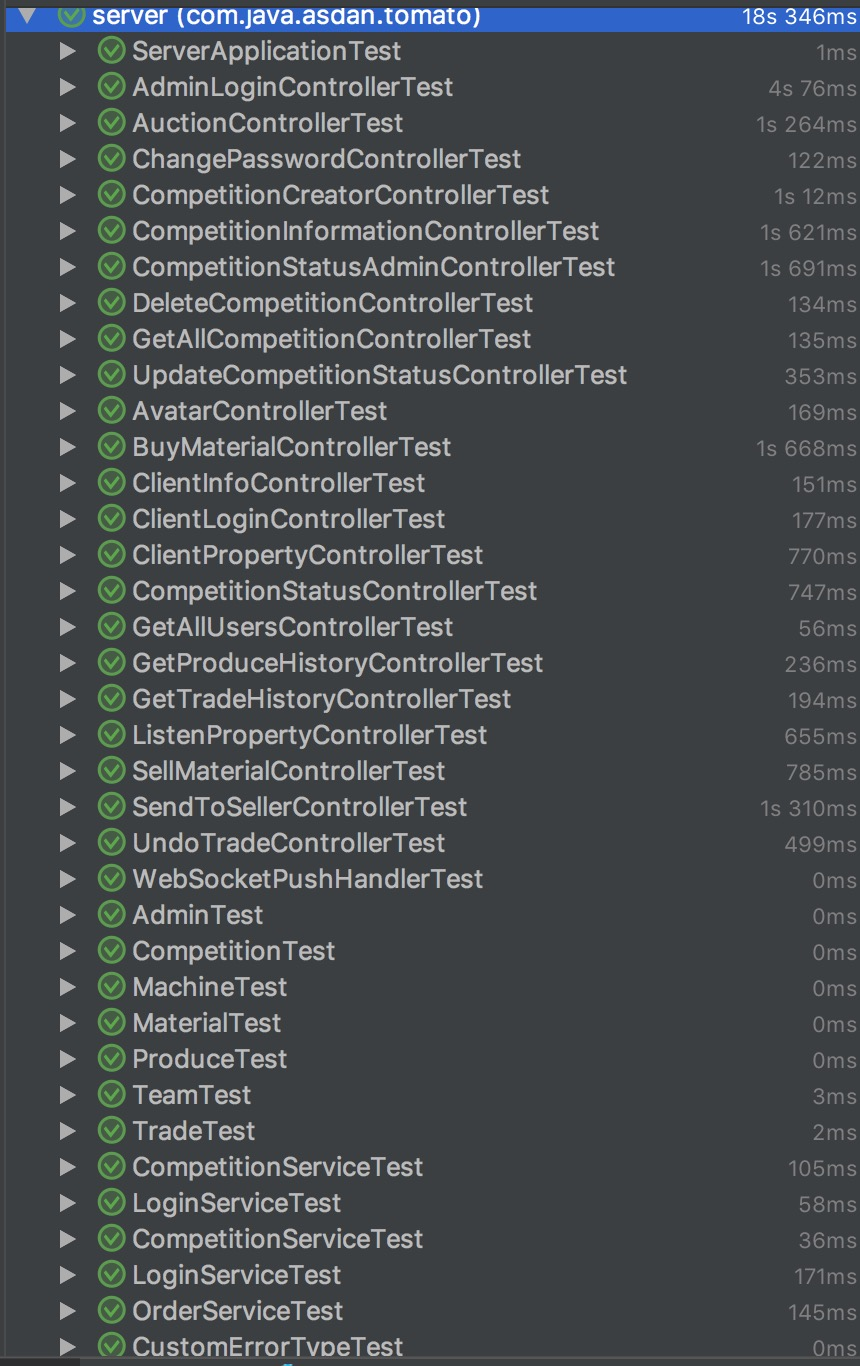
\includegraphics[scale = .3]{fig/test_total_time.jpeg}
\subsection{需求的可追踪性}
本测试计划覆盖了所有后端(除微信WebSocket外)的需求(接口)。
\subsection{评价}
\subsubsection{评价准则}
Coverage。
\subsubsection{数据处理}
数据处理由IntelliJ自动完成,IntelliJ将为我们生成完整的Coverage报告。
\subsubsection{结论}
本测试计划十分合理。
\subsection{注解}
% \section{软件测试说明}
% 	%unfinished 不过感觉和测试计划东西一样???
% 	\subsection{引言}
% 		\subsubsection{标识}
% 		\subsubsection{系统概述}
% 		\subsubsection{文档概述}
% 	\subsection{引用文件}
% 	\subsection{测试准备}
% 	\subsection{测试说明}
% 	\subsection{需求的可追踪性}
\section{软件测试报告}
\subsection{引言}
\subsubsection{系统概述}
可以参见《\ref{软件测试计划}》中的系统概述。
\subsubsection{文档概述}
本文档将介绍测试的详细结果,主要是Coverage。
\subsection{测试结果概述}
\subsubsection{对被测试软件的总体评估}
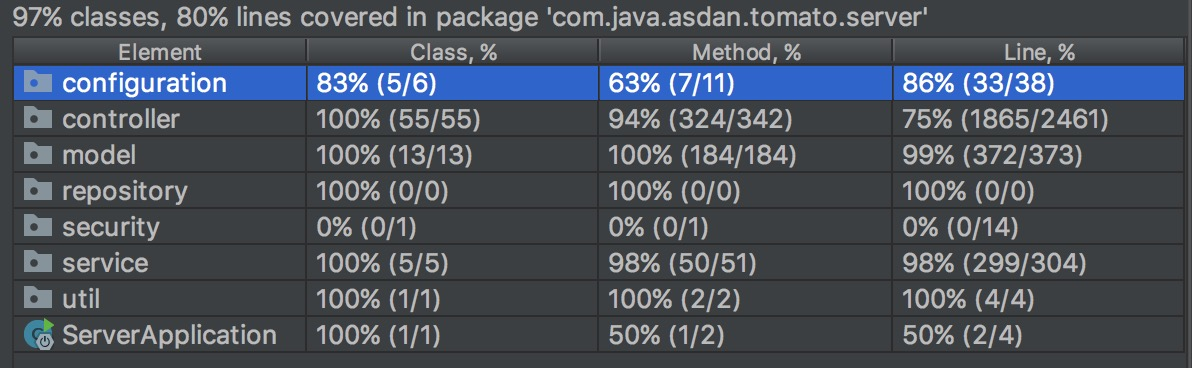
\includegraphics[scale = .3]{fig/test_1.jpg}

本测试覆盖率很高,可以说是十分到位了。
\subsubsection{测试环境的影响}
任何平台都可以进行测试,并没有什么影响。
\subsubsection{改进建议}
如果可以的话,可以绕出架构对微信的websocket进行测试。
\subsection{详细的测试结果}
以下是我们的测试覆盖率:

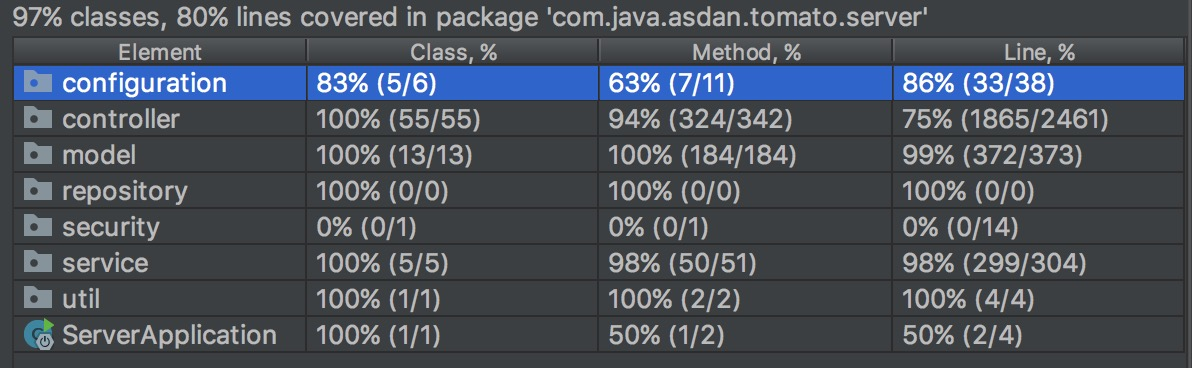
\includegraphics[scale = .3]{fig/test_1.jpg}

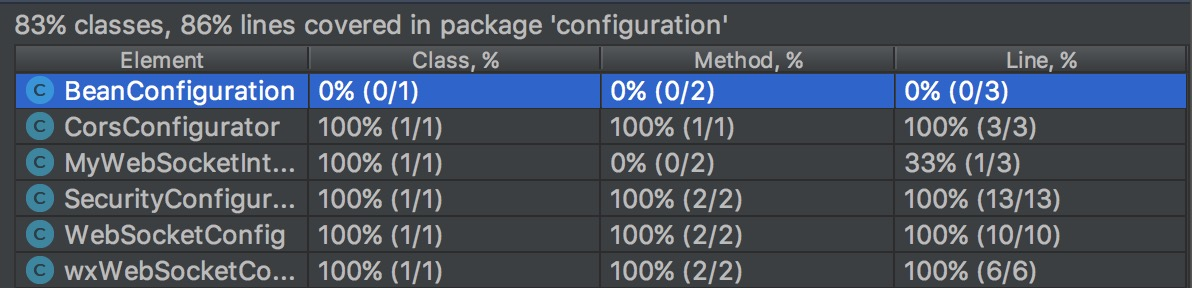
\includegraphics[scale = .3]{fig/test_2.jpg}

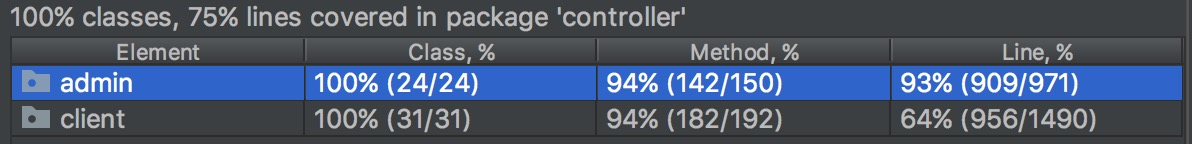
\includegraphics[scale = .3]{fig/test_3.jpg}

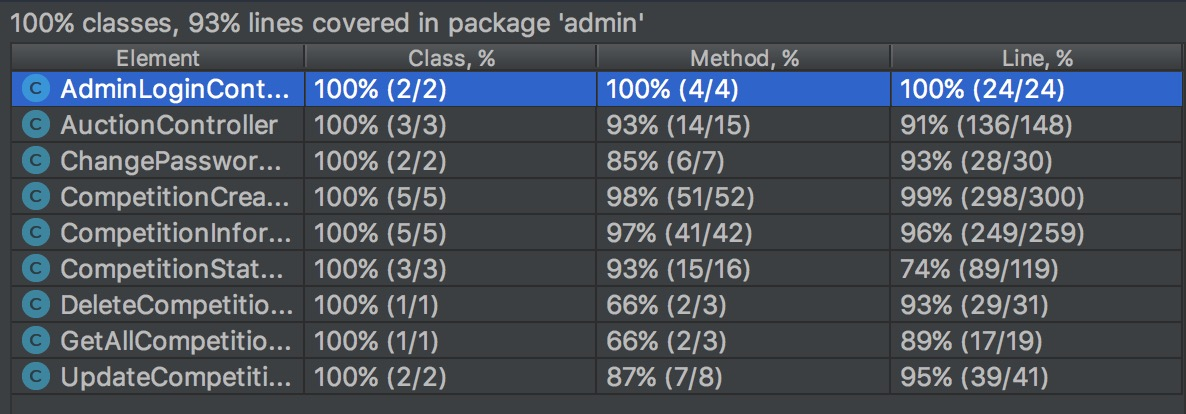
\includegraphics[scale = .3]{fig/test_4.jpg}

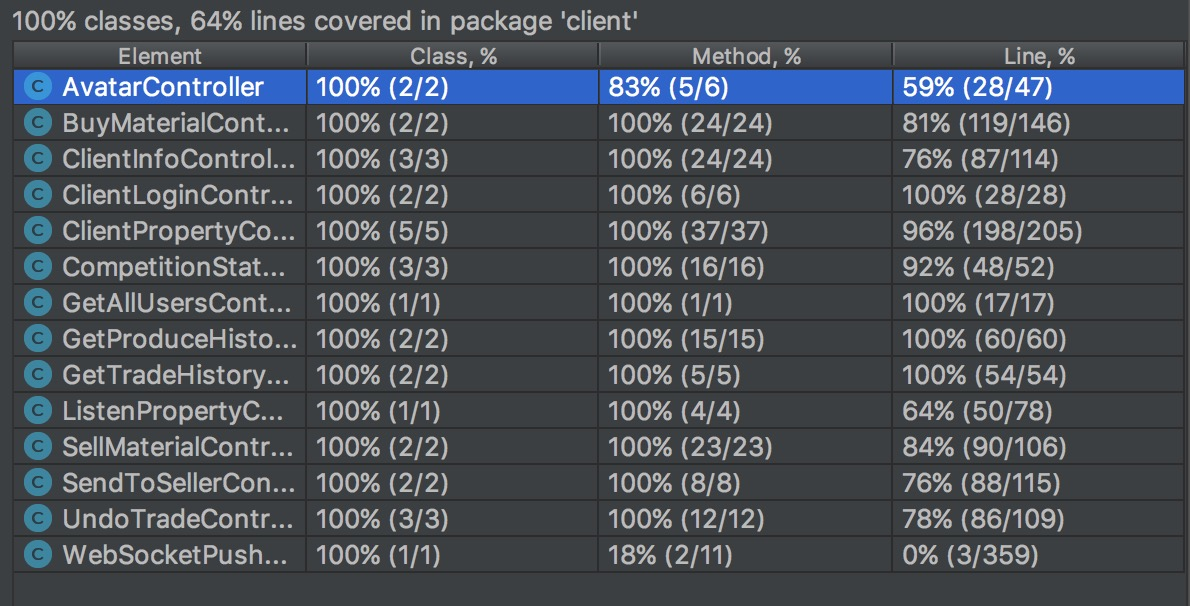
\includegraphics[scale = .3]{fig/test_5.jpg}

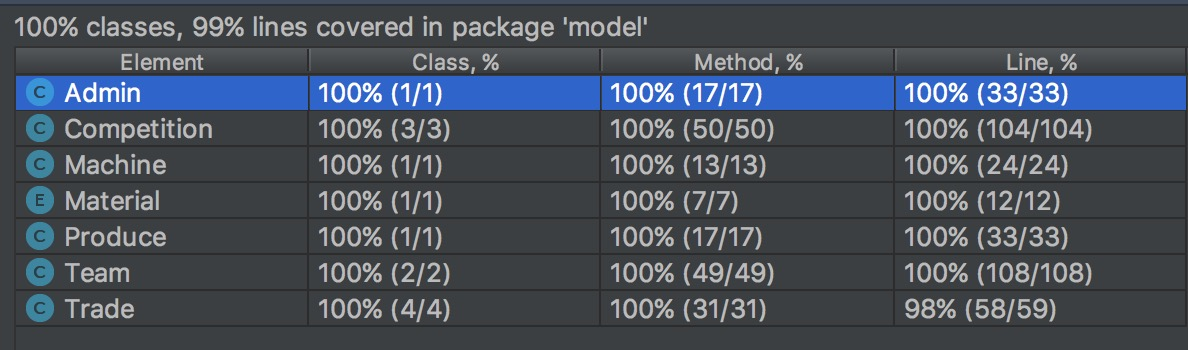
\includegraphics[scale = .3]{fig/test_6.jpg}

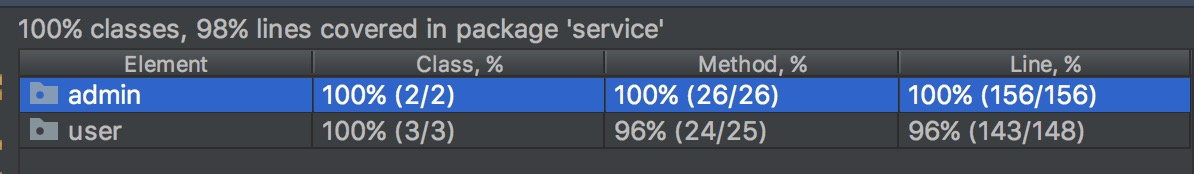
\includegraphics[scale = .3]{fig/test_7.jpg}

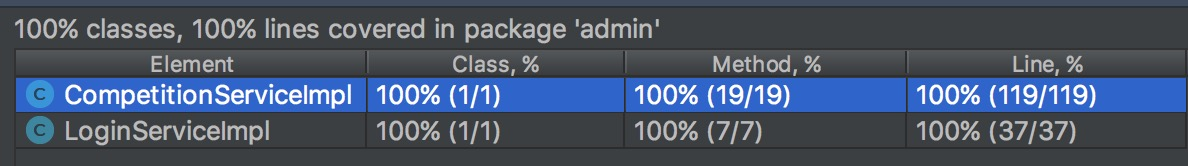
\includegraphics[scale = .3]{fig/test_8.jpg}

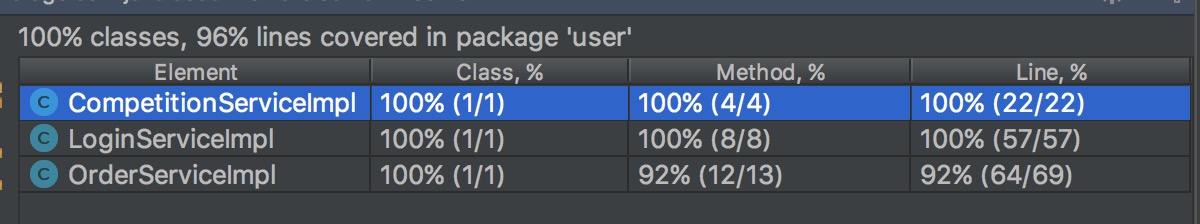
\includegraphics[scale = .3]{fig/test_9.jpg}
\subsection{测试记录}
本次测试结果生成于2018年1月19日,测试平台是Mac,集成开发环境是IntelliJ。见证者是宋世虹和张慧盟。
\subsection{评价}
\subsubsection{能力}
该测试覆盖了几乎所有后台的接口,可以说是很鲁棒,给前端提供了十分稳定的服务。
\subsubsection{缺陷和限制}
由于没有找到微信的websocket的测试方法,所以我们没有对微信的websocket进行测试,这很遗憾。同时,由于时间的关系,还有极少一部分代码没有被测试到。
\subsection{测试活动总结}
人力消耗:张慧盟、宋世虹。


\end{document}
